\documentclass{standalone}
\usepackage{tikz}
\usepackage{float}

\usepackage{graphicx}
\begin{document}
% \begin{figure}\centering

    % \end{figure}
    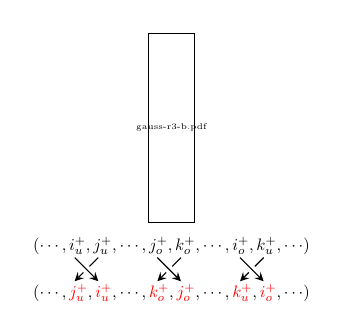
\begin{tikzpicture}[scale=.6, every node/.style={scale=.6}]
      % \pgfdeclareimage[height=4cm]{ra}{gauss-r3.pdf}
      \pgfdeclareimage[height=4cm]{rb}{gauss-r3-b.pdf}

      % \node () at (-5,4) {\pgfuseimage{ra}};
      \node () at (5,3) {\pgfuseimage{rb}};

      \def\myshift{5cm}

      \begin{scope}[xshift=\myshift]
        \node (top) at (0,.5) {$(\cdots, i_u^+, j_u^+, \cdots, j_o^+,
          k_o^+, \cdots, i_o^+, k_u^+, \cdots)$};

        \node (bot) at (0,-.5) {$(\cdots, {\color{red} j_u^+},
          {\color{red} i_u^+}, \cdots, {\color{red} k_o^+}, {\color{red}
            j_o^+}, \cdots, {\color{red} k_u^+}, {\color{red} i_o^+},
          \cdots)$};

        \begin{scope}[xshift=-.3cm]
          % Left pair
          \draw[-stealth] (-1.25, .25) -- (-1.75,-.25);
          \draw[white, line width=3pt] (-1.75, .25) -- (-1.25,-.25);
          \draw[-stealth] (-1.75, .25) -- (-1.25,-.25);

          % Center pair
          \draw[-stealth] (.5, .25) -- (0,-.25);
          \draw[white, line width=3pt] (0, .25) -- (.5,-.25);
          \draw[-stealth] (0, .25) -- (.5,-.25);

          % Right pair
          \draw[-stealth] (2.25, .25) -- (1.75,-.25);
          \draw[white, line width=3pt] (1.75, .25) -- (2.25,-.25);
          \draw[-stealth] (1.75, .25) -- (2.25,-.25);
        \end{scope}
      \end{scope}
    \end{tikzpicture}
\end{document}
